% Fig. 1 of the paper (workflow of the segmented prefilter). Compile with: pdflatex workflow_diagram.tex
\documentclass[border=2pt]{standalone}
\usepackage{mathptmx}
\usepackage{tikz}
\usetikzlibrary{arrows.meta,positioning,calc,fit,backgrounds}
\definecolor{ink}{HTML}{0B0B0B}\definecolor{ink2}{HTML}{52514E}
\definecolor{c1}{HTML}{2A78D6}\definecolor{c2}{HTML}{EB6834}\definecolor{c3}{HTML}{1BAF7A}
\begin{document}
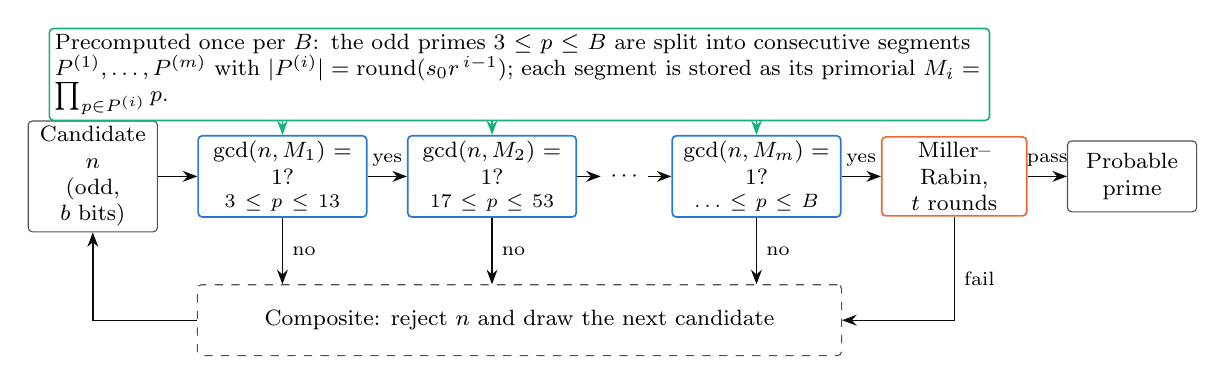
\begin{tikzpicture}[font=\footnotesize, >=Stealth, node distance=4mm and 5mm,
  box/.style={draw=ink2, rounded corners=1.5pt, align=center, minimum height=9mm, inner sep=2pt, fill=white},
  seg/.style={box, draw=c1, line width=0.6pt, text width=20mm},
  mr/.style={box, draw=c2, line width=0.6pt, text width=17mm},
  io/.style={box, text width=15mm},
  arr/.style={->, draw=ink, line width=0.5pt}]
% main pipeline
\node[io] (cand) {Candidate $n$\\ (odd, $b$ bits)};
\node[seg, right=of cand] (s1) {$\gcd(n,M_1)=1$?\\[-1pt] {\scriptsize $3\le p\le 13$}};
\node[seg, right=of s1] (s2) {$\gcd(n,M_2)=1$?\\[-1pt] {\scriptsize $17\le p\le 53$}};
\node[right=3mm of s2] (dots) {$\cdots$};
\node[seg, right=3mm of dots] (sm) {$\gcd(n,M_m)=1$?\\[-1pt] {\scriptsize $\ldots\le p\le B$}};
\node[mr, right=of sm] (mr) {Miller--Rabin,\\ $t$ rounds};
\node[io, right=of mr] (out) {Probable\\ prime};
\draw[arr] (cand) -- (s1);
\draw[arr] (s1) -- node[above,font=\scriptsize]{yes} (s2);
\draw[arr] (s2) -- (dots); \draw[arr] (dots) -- (sm);
\draw[arr] (sm) -- node[above,font=\scriptsize]{yes} (mr);
\draw[arr] (mr) -- node[above,font=\scriptsize]{pass} (out);
% reject bar
\coordinate (rl) at ($(s1.south west)+(0,-10mm)$); \coordinate (rr) at ($(sm.south east)+(0,-16mm)$);
\node[box, draw=ink2, dashed, fit=(rl)(rr), inner sep=0pt] (rej) {};\node at (rej.center) {Composite: reject $n$ and draw the next candidate};
\foreach \s in {s1,s2,sm} \draw[arr] (\s.south) -- node[right,font=\scriptsize,pos=0.5]{no} (\s.south |- rej.north);
\draw[arr] (mr.south) |- node[right,font=\scriptsize,pos=0.3]{fail} (rej.east);
\draw[arr] (rej.west) -| (cand.south);
% precomputation
\node[box, draw=c3, line width=0.6pt, above=7mm of $(s1)!0.5!(sm)$, text width=118mm, minimum height=7mm, align=left] (pre)
 {\raggedright Precomputed once per $B$: the odd primes $3\le p\le B$ are split into consecutive segments $P^{(1)},\ldots,P^{(m)}$ with $|P^{(i)}|=\mathrm{round}(s_0r^{\,i-1})$; each segment is stored as its primorial $M_i=\prod_{p\in P^{(i)}}p$.};
\foreach \s in {s1,s2,sm} \draw[->, draw=c3, line width=0.5pt] (pre.south -| \s) -- (\s.north);
\end{tikzpicture}
\end{document}
